\documentclass[]{article}
\usepackage[a4paper,top=3cm,bottom=2.5cm,left=2.5cm,
            right=2cm,marginparwidth=1.75cm,
            headheight=5pt]{geometry}
\usepackage[T5]{fontenc}
\usepackage[utf8]{inputenc}
\usepackage[document]{}
\usepackage[vietnamese]{babel}
\usepackage[unicode]{hyperref}
\usepackage{amsmath}
\usepackage{setspace}
\usepackage{graphicx}
\usepackage{caption}
\usepackage{subcaption}
\usepackage{tcolorbox}
\usepackage{listings}
\usepackage{hyperref}
\usepackage{xcolor}
\usepackage{longtable}
\usepackage{titlesec}
\usepackage{floatrow}
\usepackage[nottoc]{tocbibind}
\usepackage{mdframed}
\usepackage{amsmath}
\usepackage{amssymb}
\usepackage{tgbonum}
\usepackage{type1cm}
\usepackage{indentfirst}
\usepackage{lettrine}
\usepackage{colortbl}
\usepackage{fancyhdr}
\usepackage{wrapfig}
\usepackage{lastpage}
\usepackage{url}
\addto\captionsenglish{
  \renewcommand{\contentsname}{MỤC LỤC}%
  \renewcommand{\listfigurename}{Danh sách ảnh}%
  \renewcommand{\listtablename}{Danh sách bảng}%
  \renewcommand{\figurename}{Hình}
  \renewcommand{\tablename}{Bảng}
}
\pagestyle{fancy}
\fancyhf{}
\rhead{Toán ứng dụng và thống kê}
\lhead{\color{cyan}Đồ án 3: Linear Regression}
\lfoot{Trang \thepage /\pageref{LastPage}}
\renewcommand{\footrulewidth}{0.4pt}
\setlength{\parindent}{1.5em}
\setlength{\parskip}{1cm}
\renewcommand{\baselinestretch}{1.5}
\newmdenv[linecolor=black,skipabove=\topsep,skipbelow=\topsep,
leftmargin=2.5cm,rightmargin=2.5cm,
innerleftmargin=5cm,innerrightmargin=5cm]{mybox}
\usepackage{multicol}
\usepackage{indentfirst}
\usepackage{color}
\usepackage{tikz}
\graphicspath{{Figures/}} 
\usepackage{lipsum}
\usetikzlibrary{calc}
\setlength{\columnseprule}{2pt}
\def\columnseprulecolor{\color{black}}
\def\maru#1{\textcircled{\scriptsize#1}}

\usepackage[backend=biber, style=numeric]{biblatex}
\addbibresource{refs.bib} % Tải tệp references.bib
\defbibheading{mybibintoc}{\section{Tài liệu tham khảo}}


\begin{document}

% Bìa trang
\begin{titlepage}
\begin{tikzpicture}[remember picture,overlay,inner sep=0,outer sep=0]
     \draw[blue!70!black,line width=4pt] ([xshift=-1.5cm,yshift=-2cm]current page.north east) coordinate (A)--([xshift=2cm,yshift=-2cm]current page.north west) coordinate(B)--([xshift=2cm,yshift=2cm]current page.south west) coordinate (C)--([xshift=-1.5cm,yshift=2cm]current page.south east) coordinate(D)--cycle;

     \draw ([yshift=0.5cm,xshift=-0.5cm]A)-- ([yshift=0.5cm,xshift=0.5cm]B)--
     ([yshift=-0.5cm,xshift=0.5cm]B) --([yshift=-0.5cm,xshift=-0.5cm]B)--([yshift=0.5cm,xshift=-0.5cm]C)--([yshift=0.5cm,xshift=0.5cm]C)--([yshift=-0.5cm,xshift=0.5cm]C)-- ([yshift=-0.5cm,xshift=-0.5cm]D)--([yshift=0.5cm,xshift=-0.5cm]D)--([yshift=0.5cm,xshift=0.5cm]D)--([yshift=-0.5cm,xshift=0.5cm]A)--([yshift=-0.5cm,xshift=-0.5cm]A)--([yshift=0.5cm,xshift=-0.5cm]A);


     \draw ([yshift=-0.3cm,xshift=0.3cm]A)-- ([yshift=-0.3cm,xshift=-0.3cm]B)--
     ([yshift=0.3cm,xshift=-0.3cm]B) --([yshift=0.3cm,xshift=0.3cm]B)--([yshift=-0.3cm,xshift=0.3cm]C)--([yshift=-0.3cm,xshift=-0.3cm]C)--([yshift=0.3cm,xshift=-0.3cm]C)-- ([yshift=0.3cm,xshift=0.3cm]D)--([yshift=-0.3cm,xshift=0.3cm]D)--([yshift=-0.3cm,xshift=-0.3cm]D)--([yshift=0.3cm,xshift=-0.3cm]A)--([yshift=0.3cm,xshift=0.3cm]A)--([yshift=-0.3cm,xshift=0.3cm]A);

   \end{tikzpicture}
\newcommand{\HRule}{\rule{\linewidth}{0.5mm}}
\center

\textsc{\Large TRƯỜNG ĐẠI HỌC KHOA HỌC TỰ NHIÊN}\\[0.5cm]
\textsc{\Large KHOA CÔNG NGHỆ THÔNG TIN}\\[1cm]

\includegraphics[width=0.3\textwidth]{logo/KHTN.jpg}\\[1cm]

\HRule \\[0.4cm]
{\huge \bfseries ĐỒ ÁN 3: LINEAR REGRESSION} \\[0.4cm]
{\large TOÁN ỨNG DỤNG VÀ THỐNG KÊ}\\[0.1cm]
\HRule \\[1.5cm]

\centerline{\Large{\textbf{Triệu Nhật Minh — 21127112 — 21CLC02}}}
\vspace{2.5cm}
\centerline{\large{\textit{Giảng viên hướng dẫn}}}
\vspace{0.25cm}
\centerline{\large{Vũ Quốc Hoàng}}
\centerline{\large{Lê Thanh Tùng}}
\centerline{\large{Nguyễn Văn Quang Huy}}
\centerline{\large{Phan Thị Phương Uyên}}

\vspace{2.5cm}
\centerline{\today}


\vfill % Wipe blank space of the page.
\end{titlepage}

% Mục lục tự động
\setlength{\parskip}{.7em}
\tableofcontents
\newpage

% Table of Figures & Tables
\setlength{\parskip}{.5em}
%\listoffigures
%\listoftables
\newpage

% Bắt đầu nội dung

\section{Thư viện sử dụng}
\subsection{pandas}
Thư viện cho phép thao tác với dữ liệu dạng bảng. pandas cung cấp các đối tượng DataFrame và Series, cho phép lưu trữ, truy xuất, lọc, nhóm, biến đổi và thống kê dữ liệu một cách hiệu quả và dễ dàng. Trong đồ án này, pandas được sử dụng để đọc dữ liệu từ file csv và lưu trữ dữ liệu dưới dạng DataFrame.

\subsection{numpy}
Thư viện cho phép thao tác với mảng nhiều chiều. Với bài toán data fitting sử dụng phương pháp bình phương tối thiểu (OLS Linear Regression), để giải nghiệm \textit{x} cho hệ phương trình được tính bằng công thức $\text{x} = (\text{A}^\text{T} \text{A})^{-1} \text{A}^\text{T} \text{b}$. Nhằm tối ưu thời gian tính toán, ta sử dụng hàm có sẵn từ thư viện này. Hầu hết các hàm có sẵn đã quen thuộc từ những đồ án trước, duy có hàm \textit{numpy.ravel} và \textit{numpy.triu} sẽ được giải thích rõ hơn ở phần liệt kê hàm.

\subsection{matplotlib}
Thư viện matplotlib (cụ thể là module pyplot) cho phép ta tạo ra các biểu đồ dạng 2D. matplotlib.pyplot cũng cho phép điều chỉnh các thuộc tính của đồ thị, như màu sắc, kích thước, chú thích và tiêu đề cho đồ thị. 

\subsection{seaborn}
Thư viện cho phép vẽ heatmap. Heatmap là một loại biểu đồ 2D biểu diễn giá trị của một ma trận bằng cách sử dụng các ô có màu sắc khác nhau. seaborn cung cấp các hàm để vẽ heatmap từ các đối tượng DataFrame hoặc numpy array, cũng như điều chỉnh các thuộc tính như bản đồ màu, khoảng giá trị, nhãn và tiêu đề. Heatmap là thành phần không thể thiếu để tìm hiểu mối quan hệ giữa các biến trong bộ dữ liệu và là tiền đề để thực hiện tìm mô hình cho yêu cầu 1d.

\subsection{sklearn}
Thư viện cho phép chia dữ liệu thành các fold để thực hiện cross-validation. Cross-validation là một kỹ thuật kiểm tra hiệu năng của mô hình học máy bằng cách sử dụng một phần của dữ liệu làm tập kiểm tra và phần còn lại làm tập huấn luyện. \textit{sklearn.model\_selection.KFold} cho phép chia dữ liệu thành k fold có kích thước bằng nhau và lặp qua từng fold để sử dụng làm tập kiểm tra hoặc tập huấn luyện.

\textit{sklearn.model\_selection.KFold} là một lớp trong thư viện scikit-learn, cung cấp các chỉ số để chia dữ liệu thành các tập huấn luyện và kiểm tra. Nó chia tập dữ liệu thành k fold liên tiếp. Mỗi fold được sử dụng một lần làm tập kiểm tra trong khi các fold còn lại được sử dụng làm tập huấn luyện.

Hàm tự cài đặt có thể thực hiện chức năng tương tự như KFold, nhưng có thể khác biệt về hiệu suất và tính năng. Việc sử dụng KFold từ scikit-learn có thể đảm bảo tính ổn định và độ tin cậy của kết quả, do nó được sử dụng rộng rãi trong cộng đồng khoa học dữ liệu, nhất là khi bộ dữ liệu được sử dụng trong đồ án khó có thể kiểm tra thủ công. Tuy nhiên, một hàm tự cài đặt có thể được tùy chỉnh để phù hợp với nhu cầu đặc biệt của người dùng, thậm chí có thể có hiệu suất tốt hơn so với KFold trong một số ít trường hợp.

\subsection{IPython}
Thư viện này không đóng góp vào việc giải quyết bài toán, nhưng vẫn được sử dụng vì khả năng hiển thị ngôn ngữ \LaTeX \space để trình bày công thức hồi quy tuyến tính cho yêu cầu 1a do số lượng biến lớn. Module IPython.display.Latex cho phép chèn các biểu thức \LaTeX \space vào Jupyter Notebook.

\section{Hàm sử dụng}
% Template
% \noindent
% \textbf{Input:} \\
% \textbf{Output:}
% \paragraph{Mô tả:}
\subsection{Hàm built-in từ thư viện}
% Pandas
\subsubsection{Hàm pandas.read\_csv}
\noindent
\textbf{Input:} Đường dẫn đến file csv. \\
\textbf{Output:} DataFrame chứa dữ liệu từ file csv.
\paragraph{Mô tả:}

Hàm \textit{pandas.read\_csv} \cite{pandasreadcsv} được sử dụng để đọc dữ liệu từ file csv và lưu trữ dữ liệu dưới dạng DataFrame. Hàm này có thể nhận thêm các tham số để tùy chỉnh cách đọc dữ liệu, nhưng trong đồ án này ta giữ nguyên các tham số khác xem như mặc định, chỉ tùy chỉnh đường dẫn đến file csv.

\subsubsection{Hàm pandas.drop}
\noindent
\textbf{Input:} Tên cột cần xóa. \\
\textbf{Output:} DataFrame sau khi đã xóa cột.

\paragraph{Mô tả:}
Trong yêu cầu 1d, để xây dựng mô hình chứa các đặc trưng chứa ít sự tương quan nhát (least correlation features), sau khi đã tìm được ma trận tương quan giữa các cột, ta sẽ xóa các cột có độ tương quan cao hơn 0.6. Mặc dù trong cộng đồng khoa học dữ liệu, các đặc trưng có độ tương quan cao hơn 0.95 mới được xem là có sự tương quan cao, nhưng trong đồ án này, dựa vào ma trận tương quan thì giá trị lớn nhất là 0.64 nên ta sẽ xóa các cột có độ tương quan cao hơn 0.6. Và hàm \textit{pandas.drop} \cite{pydataPandasDataFramedrop} được gọi để xóa cột dựa trên tên cột thoả yêu cầu đã đề cập.

\begin{figure}[!h]
    \centering
    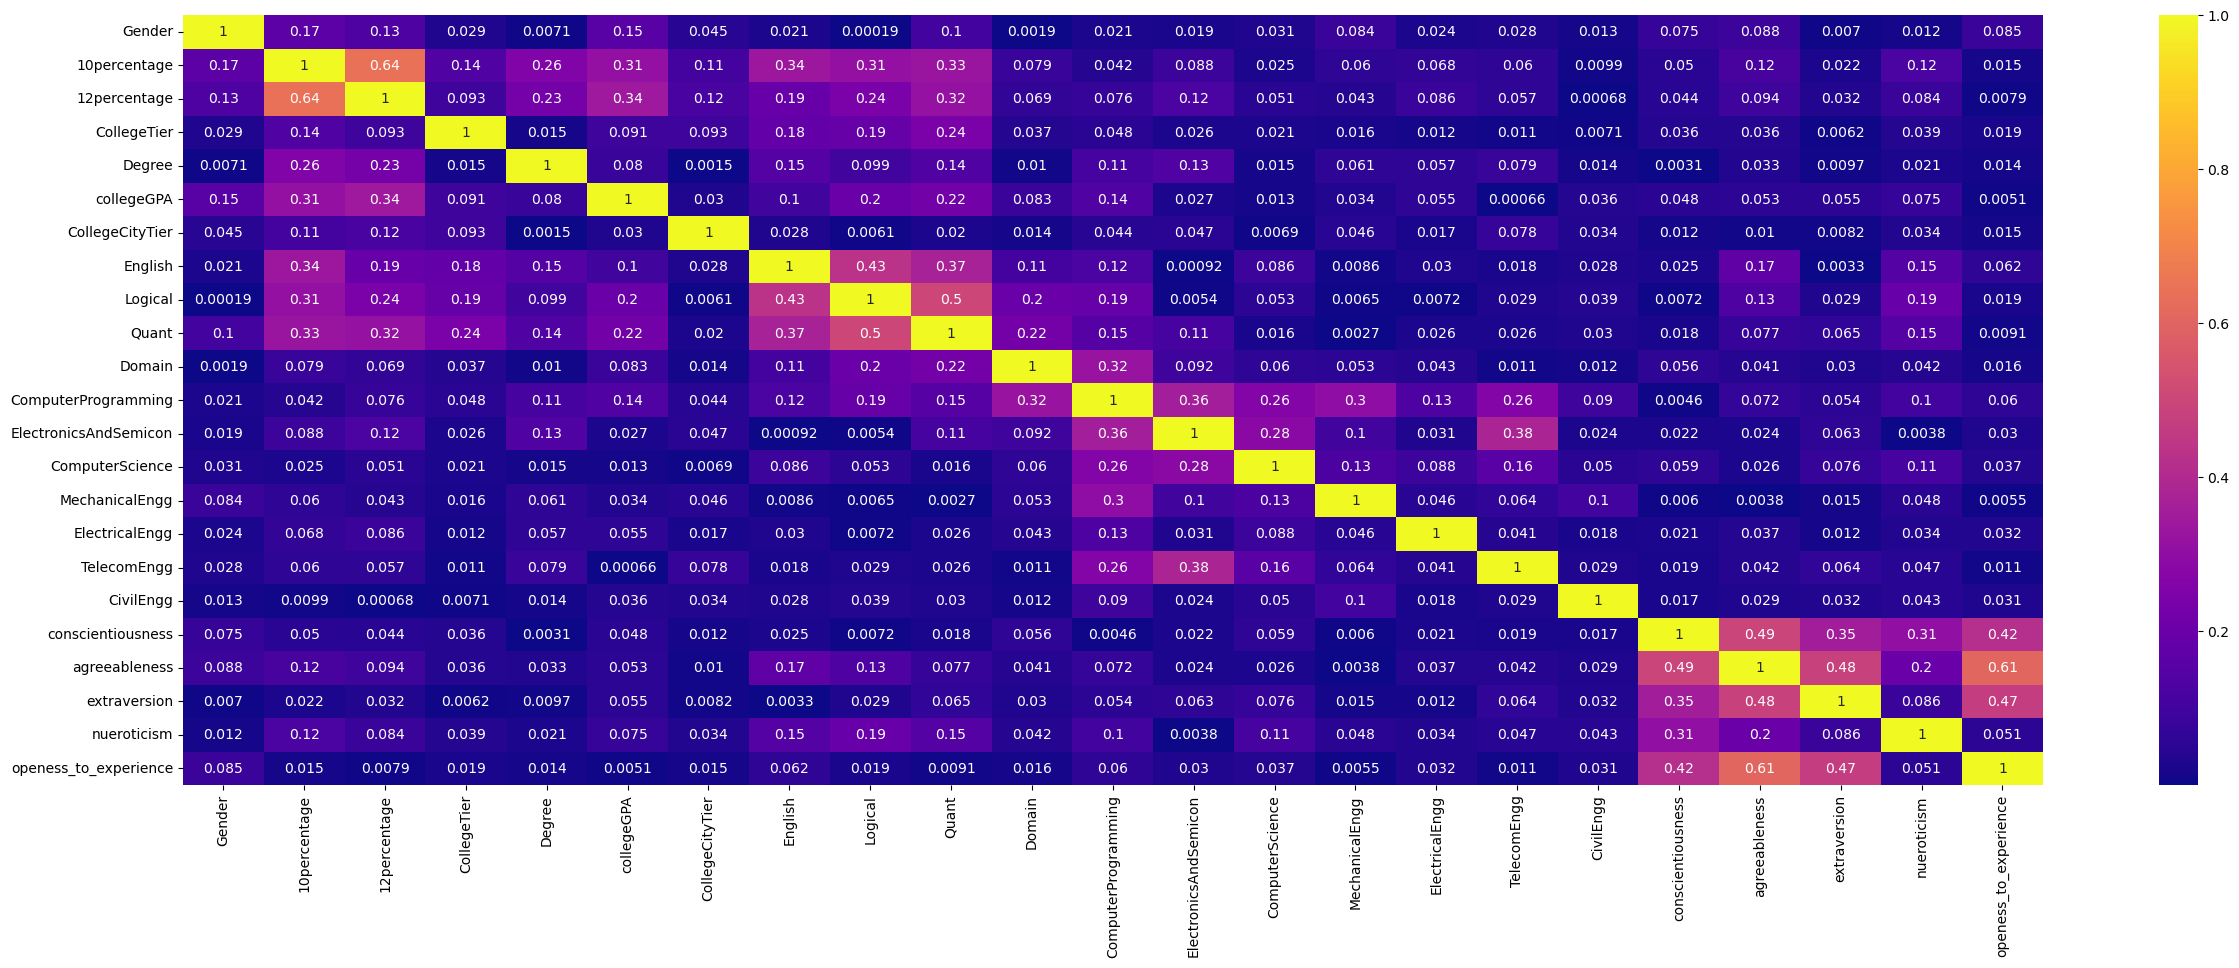
\includegraphics[width=\textwidth]{image/heatmap.png}
    \caption{Ma trận tương quan giữa các cột trong yêu cầu 1d}
    \label{fig:1d_corr}
\end{figure}

\subsubsection{Hàm pandas.corr}
\noindent
\textbf{Input:} Các tham số để tùy chỉnh cách tính ma trận tương quan. \\
\textbf{Output:} DataFrame chứa ma trận tương quan giữa các cột.
\paragraph{Mô tả:}

Ma trận tương quan (correlation matrix) là một ma trận vuông chứa các hệ số tương quan giữa nhiều biến. Mỗi ô trong bảng cho biết mối tương quan giữa hai biến cụ thể. Ma trận tương quan thường được sử dụng để tóm tắt dữ liệu, làm đầu vào cho phân tích nâng cao hơn và làm chẩn đoán cho phân tích nâng cao

Một số điểm cần lưu ý khi đọc ma trận tương quan:
\begin{itemize}
  \item Các hệ số tương quan trên đường chéo của bảng đều bằng 1 vì mỗi biến hoàn toàn tương quan với chính nó.
  \item Chỉ một nửa của ma trận tương quan cần được hiển thị vì nửa còn lại của các hệ số tương quan trong ma trận là dư thừa và không cần thiết.
  \item Ta có thể tô màu ma trận tương quan sẽ được như một bản đồ nhiệt (sử dụng tham số \textit{cmap} trong hàm heatmap) để làm cho các hệ số tương quan dễ đọc hơn.
\end{itemize}

Trong đồ án này, phương pháp Pearson \cite{wikipediaPearsonCorrelation} được sử dụng để tính ma trận tương quan. Phương pháp này được sử dụng để đo lường mối quan hệ giữa hai biến ngẫu nhiên X và Y. Giá trị của hệ số tương quan Pearson nằm trong khoảng [-1, 1]. Hệ số tương quan bằng 1 nếu có mối quan hệ tuyến tính thuận hoàn hảo giữa hai biến, bằng -1 nếu có mối quan hệ tuyến tính nghịch hoàn hảo giữa hai biến. Hệ số tương quan bằng 0 nếu không có mối quan hệ tuyến tính giữa hai biến.

Công thức tính hệ số tương quan Pearson giữa hai biến X và Y:
\begin{equation}
    \text{r}_{\text{X,Y}} = \frac{\sum_{i=1}^{n} (x_i - \bar{x})(y_i - \bar{y})}{\sqrt{\sum_{i=1}^{n} (x_i - \bar{x})^2} \sqrt{\sum_{i=1}^{n} (y_i - \bar{y})^2}}
\end{equation}

Trong đó:
\begin{itemize}
    \item $\text{r}_{\text{X,Y}}$ là hệ số tương quan Pearson giữa hai biến X và Y.
    \item $x_i$ là giá trị của biến X tại điểm dữ liệu thứ i.
    \item $y_i$ là giá trị của biến Y tại điểm dữ liệu thứ i.
    \item $\bar{x}$ là giá trị trung bình của biến X.
    \item $\bar{y}$ là giá trị trung bình của biến Y.
    \item n là số lượng điểm dữ liệu.
\end{itemize}

Do ta cần quan tâm độ tương quan giữa hai đặc trưng chứ không quan tâm chúng có tương quan thuận hay nghịch, nên ta sẽ lấy giá trị tuyệt đối của hệ số tương quan Pearson để tính ma trận tương quan. Bằng cách gọi hàm \textit{abs()} trên DataFrame chứa ma trận tương quan, ta sẽ được ma trận tương quan giữa các cột như hình 

% Numpy
\subsubsection{Hàm numpy.linalg.inv}
\noindent
\textbf{Input:} Ma trận vuông cần tính ma trận nghịch đảo. \\
\textbf{Output:} Ma trận nghịch đảo của ma trận đầu vào.
\paragraph{Mô tả:}

Hàm \textit{numpy.linalg.inv} \cite{numpyNumpylinalginv} được sử dụng để tính ma trận nghịch đảo của ma trận vuông. Trong đồ án này, hàm này được sử dụng để tính ma trận nghịch đảo của ma trận $\text{A}^\text{T} \text{A}$ để tìm nghiệm của hệ phương trình tuyến tính $\text{x} = (\text{A}^\text{T} \text{A})^{-1} \text{A}^\text{T} \text{b}$ (hàm \textit{fit} trong class OLSLinearRegression tự cài đặt, song để tối ưu hoá thời gian tính toán, ta sẽ sử dụng hàm \textit{numpy.linalg.inv} để tính ma trận nghịch đảo thay vì tự cài đặt).

\subsubsection{Hàm numpy.ravel} \label{ravel}
\noindent
\textbf{Input:} Mảng NumPy được đọc theo thứ tự được chỉ định bởi tham số order và được đóng gói thành một mảng 1 chiều và được đọc theo thứ tự C. \\
\textbf{Output:} Mảng NumPy một chiều.
\paragraph{Mô tả:}

Trong numpy, tham số order được sử dụng để chỉ định cách mà các phần tử của một mảng được lưu trữ trong bộ nhớ C trong \textit{order='C'}, có nghĩa là mảng được lưu trữ theo thứ tự liên tục của C, hay chỉ số cuối cùng thay đổi nhanh nhất \cite{stackoverflowCOrder}. Điều này có nghĩa là khi bạn duyệt qua các phần tử của một mảng nhiều chiều theo thứ tự C, bạn sẽ duyệt qua các phần tử của chỉ số cuối cùng trước, sau đó tăng chỉ số kế cuối lên 1 và tiếp tục duyệt qua các phần tử của chỉ số cuối cùng, và cứ tiếp tục như vậy cho đến khi duyệt hết các phần tử của mảng.

Trong bài toán hồi quy tuyến tính, chúng ta cần tìm một ma trận trọng số self.w sao cho tổng bình phương sai số giữa giá trị dự đoán và giá trị thực tế là nhỏ nhất. Để làm được điều này, chúng ta cần biến đổi ma trận trọng số thành một vector có kích thước bằng với số lượng tham số trong mô hình. Hàm \textit{numpy.ravel()} \cite{numpyNumpyravel} giúp chúng ta thực hiện việc này một cách dễ dàng và nhanh chóng. Bằng cách sử dụng hàm này, chúng ta có thể tính toán tích vô hướng giữa vector trọng số và ma trận đầu vào X bằng cách nhân từng phần tử tương ứng và cộng lại bằng cách gọi hàm \textit{numpy.sum}. Cuối cùng ta thu được giá trị dự đoán cho từng quan sát trong ma trận đầu vào X.

Hàm \textit{numpy.ravel} cũng được sử dụng trong hàm \ref{mae} để làm phẳng các mảng đầu vào y và y\_hat thành các mảng 1 chiều. Điều này cho phép tính toán trực tiếp sự khác biệt tuyệt đối giữa các phần tử tương ứng của hai mảng bằng cách trừ chúng và lấy giá trị tuyệt đối. Sau đó, giá trị trung bình của các sự khác biệt tuyệt đối được tính toán bằng hàm \textit{numpy.mean} để trả về giá trị lỗi trung bình tuyệt đối (MAE) giữa hai mảng.

\subsubsection{Hàm numpy.sum}
\noindent
\textbf{Input:} Mảng NumPy cần tính tổng, cột cần tính tổng \\
\textbf{Output:} Hàm này trả về kết quả là tổng của các phần tử trong mảng đầu vào theo các tham số đã xác định. Hàm có thể xử lý các mảng có kích thước và chiều khác nhau, và có thể thực hiện broadcasting nếu các kích thước tương thích.
\paragraph{Mô tả:}

Hàm \textit{numpy.sum} \cite{numpyNumpysum} được sử dụng để tính tổng các phần tử trong mảng. Trong đồ án này, hàm này được sử dụng để tính tổng các phần tử trong mảng đầu vào X bằng cách nhân từng phần tử tương ứng của vector trọng số và ma trận đầu vào X và cộng lại. Cuối cùng ta thu được giá trị dự đoán cho từng quan sát trong ma trận đầu vào X.
 
\subsubsection{Hàm numpy.mean} \label{mean}
\noindent
\textbf{Input:} Mảng NumPy cần tính trung bình, cột cần tính trung bình \\
\textbf{Output:} Hàm này trả về kết quả là trung bình của các phần tử trong mảng đầu vào theo các tham số đã xác định. Hàm có thể xử lý các mảng có kích thước và chiều khác nhau, và có thể thực hiện broadcasting nếu các kích thước tương thích.
\paragraph{Mô tả:}
Hàm \textit{numpy.mean} \cite{numpyNumpymean} được sử dụng để tính giá trị trung bình của các phần tử trong mảng. Trong đồ án này, hàm này được sử dụng để tính giá trị trung bình của các sự khác biệt tuyệt đối giữa các phần tử tương ứng của hai mảng bằng cách trừ chúng và lấy giá trị tuyệt đối. Sau đó, giá trị trung bình của các sự khác biệt tuyệt đối được tính toán bằng hàm \textit{numpy.mean} để trả về giá trị lỗi trung bình tuyệt đối (MAE) giữa hai mảng.

\subsubsection{Hàm numpy.triu}
\noindent
\textbf{Input:} Mảng NumPy cần tìm ma trận tam giác trên, kích thước của ma trận tam giác trên \\
\textbf{Output:} Mảng NumPy chứa ma trận tam giác trên của mảng đầu vào.
\paragraph{Mô tả:}
Hàm này trả về một bản sao của mảng đầu vào với các phần tử dưới đường chéo thứ k bị đưa về 0. Đối với các mảng có số chiều lớn hơn 2, triu sẽ áp dụng cho hai trục cuối cùng \cite{numpyNumpytriu}.

\subsubsection{Hàm numpy.where}
\noindent
\textbf{Input:} Mảng NumPy cần tìm vị trí, giá trị cần tìm vị trí \\
\textbf{Output:} Mảng NumPy chứa các vị trí của giá trị cần tìm.
\paragraph{Mô tả:}

Hàm \textit{numpy.where} \cite{numpyNumpywhere} được sử dụng để lọc các phần tử của một mảng dựa trên một điều kiện cho trước. Cụ thể hơn, \textcolor{red}{\textit{np.triu(np.ones(corr\_matrix.shape), k=1).astype(bool)}} sẽ tạo ra một mảng có cùng kích thước với corr\_matrix, trong đó các phần tử nằm trên đường chéo chính (k=1) sẽ có giá trị là True, còn các phần tử còn lại có giá trị là False.

Sau đó, mảng này được sử dụng như một mặt nạ để lọc các phần tử của corr\_matrix bằng cách sử dụng phương thức where. Kết quả cuối cùng là một mảng mới chỉ chứa các phần tử nằm trên đường chéo chính của corr\_matrix, còn các phần tử còn lại sẽ bị loại bỏ (có giá trị là NaN).

Nói cách khác, đoạn code trên lọc ra ma trận tam giác trên của ma trận tương quan corr\_matrix, loại bỏ các phần tử nằm dưới đường chéo chính và giữ lại các phần tử nằm trên đường chéo chính.

\subsubsection{Hàm numpy.ones}
\noindent
\textbf{Input:} Kích thước của mảng, kiểu dữ liệu của mảng \\
\textbf{Output:} Mảng NumPy chứa các phần tử có giá trị là 1.
\paragraph{Mô tả:}

Hàm \textit{numpy.ones} \cite{numpyNumpyones} được sử dụng để tạo ra một mảng có kích thước và kiểu dữ liệu nhất định, trong đó các phần tử có giá trị là 1.

% Seaborn
\subsubsection{Hàm seaborn.heatmap}
\noindent
\textbf{Input:} Ma trận tương quan, các tham số để tùy chỉnh cách vẽ heatmap. \\
\textbf{Output:} Biểu đồ heatmap.
\paragraph{Mô tả:}

Hàm \textit{seaborn.heatmap} \cite{pydataSeabornheatmap} được sử dụng để vẽ heatmap từ các đối tượng DataFrame hoặc numpy array, cũng như điều chỉnh các thuộc tính như bản đồ màu, khoảng giá trị, nhãn và tiêu đề. Heatmap là thành phần không thể thiếu để tìm hiểu mối quan hệ giữa các biến trong bộ dữ liệu và là tiền đề để thực hiện tìm mô hình cho yêu cầu 1d.

Tham số \textit{annot} trong hàm \textit{sns.heatmap} được sử dụng để kiểm soát việc hiển thị giá trị của các ô trong biểu đồ heatmap. Nếu \textit{annot=True}, thì giá trị của mỗi ô sẽ được hiển thị bên trong ô đó.

Biểu đồ heatmap với ma trận tương quan \text{corr\_matrix}, sử dụng bản đồ màu plasma, và hiển thị giá trị của mỗi ô bên trong ô đó. Nếu tham số này là False, thì giá trị của mỗi ô sẽ không được hiển thị bên trong ô đó, chỉ hiển thị các màu tương ứng với giá trị của ô đó.

% Sklearn
\subsubsection{Lớp sklearn.model\_selection.KFold}
\noindent
\textbf{Input:} Các tham số để tùy chỉnh cách chia dữ liệu. \\
\textbf{Output:} Đối tượng KFold chứa các chỉ số để chia dữ liệu thành các tập huấn luyện và kiểm tra.
\paragraph{Mô tả:} 
Chiến lược phổ biến nhất trong học máy là chia tập dữ liệu thành tập huấn luyện và tập kiểm tra. Tỷ lệ chia có thể là 70:30 hoặc 80:20 \cite{r1}. Một trong số những phương pháp là sử dụng k-fold Cross Validation. \cite{mediumCrossValidationUsing}

Trong đồ án này, lớp \textit{sklearn.model\_selection.KFold} \cite{scikitlearnSklearnmodel} được sử dụng để chia dữ liệu thành các fold. Nó có thể nhận thêm các tham số để tùy chỉnh cách chia dữ liệu, nhưng trong đồ án này ta giữ nguyên các tham số khác xem như mặc định, chỉ tùy chỉnh số lượng fold, kiểu chia dữ liệu và trộn dữ liệu trước khi chia (lần lượt các tham số \textit{n\_splits}, \textit{shuffle} và \textit{random\_state}). Tham số \textit{n\_splits} được sử dụng để chỉ định số lượng fold (k = 20 với các yêu cầu 1b, 1c, 1d), tham số \textit{shuffle} được sử dụng để chỉ định cách chia dữ liệu, và tham số \textit{random\_state} được sử dụng để chỉ định cách trộn dữ liệu trước khi chia.

Tham số \textit{shuffle} được sử dụng để chỉ định cách chia dữ liệu. Nếu \textit{shuffle=True}, thì dữ liệu sẽ được trộn ngẫu nhiên trước khi chia. Nếu \textit{shuffle=False}, thì dữ liệu sẽ không được trộn ngẫu nhiên trước khi chia. Trong đồ án này, ta sử dụng \textit{shuffle=True} để trộn dữ liệu ngẫu nhiên trước khi chia.

Đến với tham số \textit{random\_state}, nếu \textit{random\_state=None}, thì mỗi lần chạy, lớp \textit{KFold} sẽ cho ra kết quả khác nhau. Trên thực tế, việc truyền bất kì số nguyên nào (kể cả số 0) thì cũng không thành vấn đề. Đây là một random seed trong thuật toán random của máy tính. \cite{wikipediaRandomSeed} Các thí nghiệm có cùng random seed và cùng các tham số khác sẽ cho ra kết quả giống nhau. 42 là một con số đến từ cuốn sách Hướng dẫn du lịch vũ trụ. Câu trả lời cho cuộc sống vũ trụ và mọi thứ và được coi là một trò đùa. Nó không có ý nghĩa khác ngoài việc là một con số ngẫu nhiên. \cite{stackoverflowRandomState} Trong đồ án này, ta sử dụng \textit{random\_state=42} để đảm bảo kết quả của các thí nghiệm là nhất quán.

Việc chia dữ liệu thành k phần giúp chúng ta có thể kiểm tra độ chính xác và ổn định của mô hình trên nhiều tập dữ liệu khác nhau, tránh hiện tượng quá khớp (overfitting) hoặc thiếu khớp (underfitting) mô hình. Việc lựa chọn giá trị k trong k-fold cross validation là tùy thuộc vào nhiều yếu tố. Một giá trị k lớn sẽ cho phép mô hình được huấn luyện trên nhiều dữ liệu hơn, nhưng cũng sẽ tăng thời gian tính toán. Một giá trị k nhỏ sẽ giảm thời gian tính toán, nhưng cũng có thể làm tăng sai số trong việc đánh giá hiệu suất của mô hình. \cite{stackexchangeChoiceKfold}

% IPython
\subsubsection{Hàm IPython.display.Latex}
\noindent
\textbf{Input:} Chuỗi kí tự cần hiển thị ở dạng \LaTeX. \\
\textbf{Output:} Hiển thị chuỗi kí tự ở dạng \LaTeX.

\subsection{Hàm tự cài đặt}
\subsubsection{Hàm OLSLinearRegression.fit} \label{fit}
\noindent
\textbf{Input:} Ma trận chứa các giá trị của đặc trưng, y là một vector chứa các giá trị của biến mục tiêu. \\
\textbf{Output:} Chính nó (self) để có thể gọi phương thức khác trên cùng đối tượng OLSLinearRegression.
\paragraph{Mô tả:}

Hàm này sử dụng phương pháp bình phương nhỏ nhất để tính toán trọng số \textit{w} cho mô hình tuyến tính. Đầu tiên, nó tính toán ma trận giả nghịch đảo của ma trận $\text{A}^\text{T} \text{A}$ bằng hàm \textit{numpy.linalg.inv} (thay vì tự cài đặt để tối ưu hoá thời gian tính toán). 

Mục đích hàm fit của lớp OLSLinearRegression là tìm ra ma trận trọng số \textit{w} ứng với mô hình tuyến tính. Để làm được điều này, ta cần giải hệ phương trình tuyến tính $\text{A}^\text{T} \text{A} \textit{w} = \text{A}^\text{T} \text{b}$ để tìm ra giá trị của \textit{w}. Để giải hệ phương trình này, ta nhân cả hai vế của phương trình với ma trận nghịch đảo của ma trận $\text{A}^\text{T} \text{A}$, ta được $\textit{w} = (\text{A}^\text{T} \text{A})^{-1} \text{A}^\text{T} \text{b}$. Do đó, ta sẽ tính ma trận nghịch đảo của ma trận $\text{A}^\text{T} \text{A}$ bằng hàm \textit{numpy.linalg.inv} và nhân với ma trận $\text{A}^\text{T} \text{b}$ để tìm ra giá trị của \textit{w}.

\subsubsection{Hàm OLSLinearRegression.predict}
\noindent
\textbf{Input:} Ma trận chứa các giá trị của đặc trưng. \\
\textbf{Output:} Mảng NumPy chứa các giá trị dự đoán.
\paragraph{Mô tả:} 
Trong hàm \textit{predict}, ta tính toán giá trị dự đoán bằng cách nhân ma trận X với vector trọng số w (được tính toán trong hàm \hyperref{fit}{fit}) và cộng các giá trị lại với nhau theo chiều thứ nhất (axis=1) để thu được một vector kết quả. Cụ thể, ta sử dụng phép toán \textcolor{red}{\textit{np.sum(self.w.ravel() * X, axis=1)}} để thực hiện việc này.

Sở dĩ ta phải gọi hàm \textit{ravel} được sử dụng để chuyển đổi vector trọng số \textit{w} thành một mảng 1 chiều liên tục trước khi thực hiện phép nhân với ma trận đầu vào \textit{X}. Điều này cần thiết để đảm bảo rằng kích thước của \textit{w} và \textit{X} phù hợp với nhau và phép nhân. Trái lại, nếu không sử dụng hàm \textit{ravel}, vector trọng số \textit{w} có kích thước không phù hợp và dẫn đến lỗi khi thực hiện phép nhân.

\subsubsection{Hàm OLSLinearRegression.get\_params}
\noindent
\textbf{Input:} Không có. \\
\textbf{Output:} Mảng NumPy chứa các giá trị của vector trọng số \textit{w}.
\paragraph{Mô tả:}

Hàm \textit{get\_params} được sử dụng để trả về các giá trị của vector trọng số \textit{w}. Mô hình OLSLinearRegression sau khi được huấn luyện sẽ có một vector trọng số \textit{w} duy nhất, và hàm \textit{get\_params} được sử dụng để trả về các giá trị của vector trọng số này.

\subsubsection{Hàm mae} \label{mae}
\noindent
\textbf{Input:} Vector chứa các giá trị thực tế từ tập dữ liệu cho trước, vector chứa các giá trị dự đoán tính được từ mô hình. \\
\textbf{Output:} Giá trị lỗi trung bình tuyệt đối (MAE).
\paragraph{Mô tả:}

Phương pháp bình phương tối thiểu khi sử dụng để tìm mô hình tuyến tính sẽ tìm ra mô hình có giá trị trung bình của tổng bình phương sai số là nhỏ nhất.  Tuy nhiên, trong thực tế, chúng ta thường quan tâm đến giá trị trung bình của tổng sai số tuyệt đối, hay còn gọi là lỗi trung bình tuyệt đối (MAE). MAE được tính bằng cách lấy giá trị tuyệt đối của sự khác biệt giữa các giá trị thực tế và giá trị dự đoán, sau đó lấy giá trị trung bình của các sự khác biệt tuyệt đối này.

Trong hàm mae, ta sử dụng hàm \textit{numpy.ravel} để làm phẳng các mảng đầu vào y và y\_hat thành các mảng 1 chiều. Điều này cho phép tính toán trực tiếp sự khác biệt tuyệt đối giữa các phần tử tương ứng của hai mảng bằng cách trừ chúng và lấy giá trị tuyệt đối. Sau đó, giá trị trung bình của các sự khác biệt tuyệt đối được tính toán bằng hàm \textit{numpy.mean} để trả về giá trị lỗi trung bình tuyệt đối (MAE) giữa hai mảng.

\subsubsection{Hàm latex\_text}
\noindent
\textbf{Input:} Mảng NumPy chứa các tham số của mô hình tuyến tính, từ điển chứa các tên cột tương ứng với các tham số trong mảng NumPy. \\
\textbf{Output:} Hiển thị chuỗi kí tự ở dạng \LaTeX.
\paragraph{Mô tả:}

Hàm latex\_text có hai đầu vào là params và dict. Đầu vào params là một mảng numpy chứa các tham số của mô hình tuyến tính, trong khi đầu vào dict là một từ điển chứa các tên cột tương ứng với các tham số trong params. Hàm này trả về một chuỗi \LaTeX \space biểu diễn phương trình tuyến tính của mô hình dựa trên các tham số và tên cột được cung cấp.

Trong hàm này, ta bắt đầu bằng cách khởi tạo chuỗi text với giá trị ban đầu là phần đầu của phương trình \LaTeX: Hàm latex\_text có hai đầu vào là params và dict. Đầu vào params là một mảng numpy chứa các tham số của mô hình tuyến tính, trong khi đầu vào dict là một từ điển chứa các tên cột tương ứng với các tham số trong params. Hàm này trả về một chuỗi \LaTeX \space biểu diễn phương trình tuyến tính của mô hình dựa trên các tham số và tên cột được cung cấp.

Do \LaTeX \space trên Jupyter Notebook không tự xuống dòng khi độ dài của một chuỗi vượt quá chiều rộng của trang, ta sẽ thêm đoạn mã xuống dòng mỗi 4 tên cột được hiển thị (không tính cột đầu tiên).

\subsubsection{Hàm kfold\_cross\_model} \label{kfoldcrossmodel}
\noindent
\textbf{Input:} Mảng NumPy chứa các giá trị của đặc trưng, mảng NumPy chứa các giá trị của biến mục tiêu, đối tượng KFold, mảng để lưu trữ các giá trị MAE. \\
\textbf{Output:} Không có.
\paragraph{Mô tả:}

Trong hàm này, ta sử dụng vòng lặp để duyệt qua các phần chia của dữ liệu huấn luyện khi thực hiện phương pháp kfold cross validation. Mỗi phần tử của iterator là một tuple chứa hai mảng chỉ số: \textit{train\_index} và \textit{test\_index}. Mảng \textit{train\_index} chứa các chỉ số của phần huấn luyện, trong khi mảng \textit{test\_index} chứa các chỉ số của phần kiểm tra1.

Vòng lặp \textcolor{red}{\textit{for train\_index, test\_index in kf.split(X\_train\_np)}} được sử dụng để duyệt qua các phần chia của dữ liệu huấn luyện. Đối với mỗi phần chia, ta sử dụng chỉ số của phần huấn luyện và phần kiểm tra để trích xuất dữ liệu tương ứng từ X\_train\_np và y\_train\_np. Sau đó, ta có thể huấn luyện mô hình với dữ liệu huấn luyện đã trích xuất và đánh giá hiệu suất của mô hình trên dữ liệu kiểm tra. Cuối cùng, ta thêm giá trị MAE vào danh sách mae\_arr để lưu trữ kết quả. Nếu X\_train\_np là một vector 1 chiều, ta thêm một chiều mới vào cuối bằng cách sử dụng cú pháp [:, None]. Ngược lại, ta chỉ cần trích xuất dữ liệu bình thường. Sau đó, ta huấn luyện một mô hình hồi quy tuyến tính bằng cách sử dụng phương thức fit của class OLSLinearRegression với dữ liệu huấn luyện đã trích xuất. Ta sử dụng mô hình đã huấn luyện để dự đoán giá trị đầu ra cho phần kiểm tra của dữ liệu và tính toán giá trị MAE giữa giá trị thực tế và giá trị dự đoán. Cuối cùng, ta thêm giá trị MAE vào danh sách mae\_arr để lưu trữ kết quả.

Hàm này không có giá trị trả về, nhưng nó thay đổi nội dung của danh sách mae\_arr bằng cách thêm các giá trị MAE tính toán được trong quá trình kiểm định chéo.

\subsubsection{Hàm scientific\_notation\_converter}
\noindent
\textbf{Input:} Mảng chứa các trọng số của mô hình tuyến tính. \\
\textbf{Output:} Mảng chứa các trọng số của mô hình tuyến tính ở dạng ký hiệu khoa học với 3 chữ số thập phân.
\paragraph{Mô tả:}

Trong đồ án yêu cầu ta phải trình bày mô hình dự đoán mức lương với tham số được làm tròn 3 chữ số thập phân. Ta có thể sử dụng hàm \textit{round} trong phương thức \textit{get\_params}. Song nếu làm tròn ngay từ bước huấn luyện, ta sẽ mất đi độ chính xác của mô hình. Do đó, ta sẽ sử dụng hàm \textit{scientific\_notation\_converter} để chuyển đổi các trọng số của mô hình.

Trong hàm này, ta sử dụng kỹ thuật list comprehension để duyệt qua các phần tử trong params và chuyển đổi chúng thành dạng ký hiệu khoa học (scientific notation). Đối với mỗi phần tử \textit{param} trong params, sau đó định dạng nó thành chuỗi ký hiệu khoa học với 3 chữ số thập phân bằng cách sử dụng phương thức format: \textit{''\%.3f''}. Kết quả cuối cùng là một danh sách mới chứa các chuỗi ký hiệu khoa học tương ứng với các phần tử trong params.

\section{Đánh giá kết quả mô hình}
\subsection{Thông tin cấu hình}
\begin{itemize}
  \item Bộ xử lý: AMD Ryzen 7 5800H
  \item Hệ điều hành: Windows 10 Pro 64-bit
  \item Phiên bản Python: 3.10.9
\end{itemize}
% % Template yêu cầu
% \subsubsection{Các bước thực hiện}
% \subsubsection{Công thức hồi quy}
% \subsubsection{Kết quả mô hình}
% \subsubsection{Nhận xét}
\subsection{Ghi chú}
Trước khi thực hiện tìm mô hình hồi quy tuyến tính cho tất cả yêu cầu đề bài, ta cần đọc dữ liệu từ \textit{train.csv} và \textit{test.csv} ứng với tập dữ liệu huấn luyện (\textbf{train}) và tập dữ liệu kiểm tra (\textbf{test}), đồng thời xử lý DataFrame vừa đọc được để nhận biết đâu là tập các đặc trưng (\textbf{X}) và đâu là tập biến mục tiêu (\textbf{y}). Sau đó, ta sẽ chia tập dữ liệu huấn luyện thành hai phần: tập huấn luyện (\textbf{X\_train}, \textbf{y\_train}) và tập kiểm tra (\textbf{X\_test}, \textbf{y\_test}). Do tập mục tiêu là cố định (Salary ứng với \textbf{y\_train} và \textbf{y\_test}), nên ta dùng chung hai tập này cho các câu 1a, 1b, 1c, 1d. 

Sở dĩ phải chuyển về NumPy array với tất cả DataFrame vừa đọc được là vì khi thực hiện yêu cầu tìm đặc trưng tốt nhất trong số các đặc trưng (yêu cầu 1b, 1c), ma trận đặc trưng \textit{X} chỉ có 1 cột, nên khi thực hiện các phép toán trên ma trận, ta cần mở rộng 1 chiều mới có thể thực hiện phép nhân (phương thức \textit{fit} của lớp OLSLinearRegression). Nếu không mở rộng 1 chiều mới, ta sẽ gặp lỗi khi thực hiện phép nhân.

Do đồ án yêu cầu khi sử dụng cross-validation, ta chỉ được phép xáo trộn dữ liệu 1 lần duy nhất và thực hiện trên \textit{m} mô hình \cite{hcmusLearningManagement}, ta sẽ gọi lại đối tượng KFold đã được khởi tạo trước đó để sử dụng lại các chỉ số đã được tạo ra. Điều này giúp đảm bảo rằng các chỉ số được tạo ra sẽ giống nhau trong mỗi lần chạy, từ đó đảm bảo tính nhất quán của kết quả.

\subsection{Yêu cầu 1a}
\subsubsection{Các bước thực hiện}
\begin{enumerate}
  \item Thực hiện lấy 11 đặc trưng đầu tiên đề bài cung cấp.
  \item Thực hiện chia tập dữ liệu huấn luyện thành hai phần: tập huấn luyện (\textbf{X\_1a\_train}, \textbf{y\_train}) và tập kiểm tra (\textbf{X\_test}, \textbf{y\_test}).
  \item Huấn luyện mô hình hồi quy tuyến tính với tập huấn luyện (\textbf{X\_1a\_train}, \textbf{y\_train}) thu được tập mục tiêu dự đoán (\textbf{y\_pred\_1a}).
  \item Gọi hàm \textbf{mae} để tính giá trị lỗi trung bình tuyệt đối (MAE) giữa tập mục tiêu thực tế (\textbf{y\_test}) và tập mục tiêu dự đoán (\textbf{y\_pred\_1a}).
\end{enumerate}
\subsubsection{Công thức hồi quy}
$\text{Salary} = -22756.513 \times \text{Gender} + 804.503 \times \text{10percentage} + 1294.655 \times \text{12percentage} -91781.898 \times \text{CollegeTier} + 23182.389 \times \text{Degree} + 1437.549 \times \text{collegeGPA} -8570.662 \times \text{CollegeCityTier} + 147.858 \times \text{English} + 152.888 \times \text{Logical} + 117.222 \times \text{Quant} + 34552.286 \times \text{Domain}$

\subsubsection{Kết quả mô hình}
MAE = 104863.77754033195

\subsubsection{Nhận xét}
Trong một mô hình hồi quy tuyến tính, việc thêm nhiều thuộc tính có thể giúp giảm sai số trung bình tuyệt đối (MAE) bởi vì nó cho phép mô hình nắm bắt được nhiều thông tin hơn về mối quan hệ giữa các biến độc lập và biến phụ thuộc. Tuy nhiên, điều này không phải lúc nào cũng đúng. Việc thêm quá nhiều thuộc tính có thể dẫn đến hiện tượng quá khớp (overfitting), khi đó mô hình sẽ hoạt động tốt trên dữ liệu huấn luyện nhưng không hoạt động tốt trên dữ liệu kiểm tra. Việc này giống như để mô hình ''học tủ'' các quan hệ giữa các biến độc lập và biến phụ thuộc trong dữ liệu huấn luyện, khiến cho mô hình không thể áp dụng được cho các dữ liệu mới. Do đó, cách làm này làm tăng sai số trung bình tuyệt đối (MAE) trên dữ liệu kiểm tra.

\subsection{Yêu cầu 1b}
\subsubsection{Các bước thực hiện}
\begin{enumerate}
  \item Thực hiện lấy 5 đặc trưng tính cách yêu cầu
  \item Đặt giá trị k (trong k-fold cross validation) là 20.
  \item Gọi đối tượng thuộc lớp KFold trong thư viện scikit-learn nhằm cung cấp các chỉ mục để chia dữ liệu thành các tập huấn luyện và kiểm tra. 
  \item Tạo mảng chứa các giá trị MAE ứng với mỗi đặc trưng.
  \item Lần lượt duyệt qua các đặc trưng, với mỗi đặc trưng, ta thực hiện các bước sau:
  \begin{enumerate}
    \item Gọi hàm \textbf{kfold\_cross\_model} \ref{kfoldcrossmodel} với các tham số là mảng đặc trưng tương ứng, tập mục tiêu y\_train\_np, đối tượng KFold, mảng chứa các giá trị MAE.
    \item Tính giá trị trung bình của các giá trị MAE thu được từ k-fold cross validation.
    \item Thêm giá trị trung bình của các giá trị MAE thu được vào mảng chứa các giá trị MAE.
  \end{enumerate}
  \item Tìm ra đặc trưng tốt nhất bằng cách tìm ra giá trị MAE nhỏ nhất trong mảng chứa các giá trị MAE, ở đây đặc trưng tốt nhất là \textit{nueroticism}.
  \item Với đặc trưng tốt nhất vừa tìm được, ta thực hiện các bước sau:
  \begin{enumerate}
    \item Thêm chiều mới vào cuối mảng đặc trưng bằng cách sử dụng cú pháp [:, None].
    \item Huấn luyện mô hình hồi quy tuyến tính với tập huấn luyện (\textbf{X\_1b\_best\_train}, \textbf{y\_train\_np}) thu được tập mục tiêu dự đoán (\textbf{y\_pred}). Với \textbf{X\_1b\_best\_train} là mảng đặc trưng tốt nhất vừa tìm được, \textbf{y\_train\_np} là tập mục tiêu huấn luyện. 
    \item Đánh giá mô hình với tập kiểm tra (\textbf{X\_1b\_best\_test}, \textbf{y\_test}) thu được tập mục tiêu dự đoán (\textbf{y\_pred}).
    \item Gọi hàm \textbf{mae} để tính giá trị lỗi trung bình tuyệt đối (MAE) giữa tập mục tiêu thực tế (\textbf{y\_test}) và tập mục tiêu dự đoán (\textbf{y\_pred}).
  \end{enumerate}
\end{enumerate}
\subsubsection{Công thức hồi quy}
$\text{Salary} = -56546.304 \times \text{nueroticism}$
\subsubsection{Kết quả mô hình}
\begin{table}[!h]
  \centering
  \resizebox{0.5\textwidth}{!}{%
  \begin{tabular}{|c|l|l|}
  \hline
  \multicolumn{1}{|l|}{STT} & Mô hình với 1 đặc trưng & MAE \\ \hline
  1 & conscientiousness & 306221.75562170806 \\ \hline
  2 & agreeableness & 300857.53034685535 \\ \hline
  3 & extraversion & 307059.3991665598 \\ \hline
  4 & neuroticism & 299376.1964789984 \\ \hline
  5 & openness\_to\_experience & 303054.52630103764 \\ \hline
  \end{tabular}%
  }
\end{table}
Kết quả MAE của mô hình với 1 đặc trưng tốt nhất là \textbf{291019.693226953}

\subsubsection{Nhận xét}
\begin{itemize}
  \item Các tính cách này là một phần của mô hình Big Five, một khung tham chiếu phổ biến để đánh giá nhân cách của con người. Các tính cách này được đo bằng các điểm số trong bài kiểm tra AMCAT, một cổng việc làm trực tuyến. \cite{kaggleEngineeringGraduate}
  \item Các tính cách này có thể ảnh hưởng đến mức lương và công việc của các kỹ sư tốt nghiệp ở Ấn Độ. Ví dụ, neuroticism có thể liên quan đến khả năng chịu áp lực và thích nghi với môi trường làm việc. Agreeableness có thể liên quan đến khả năng hợp tác và giao tiếp với đồng nghiệp và khách hàng. Openness\_to\_experience có thể liên quan đến khả năng sáng tạo và học hỏi những điều mới. Conscientiousness có thể liên quan đến khả năng tổ chức và quản lý thời gian. Extraversion có thể liên quan đến khả năng giao tiếp và thuyết phục.
  \item Để ý rằng MAE của agreeableness và neuroticism không chênh lệch nhau quá nhiều. \\
  Theo một số nghiên cứu, các đặc trưng tính cách có thể ảnh hưởng đến mức lương và sự thăng tiến trong công việc. Tuy nhiên, mức độ ảnh hưởng của các đặc trưng tính cách có thể khác nhau tùy thuộc vào ngành nghề và công việc cụ thể. \cite{personalityTraitsPredict}
  Một báo cáo được công bố bởi trang web tìm kiếm việc làm Joblist cho thấy những người có tính cách tự phụ (conscientiousness) có xu hướng kiếm được ít nhất 75.000 đô la Mỹ mỗi năm, trong khi những người có tính cách neuroticism có xu hướng kiếm được 34.999 đô la Mỹ hoặc ít hơn mỗi năm. Tuy nhiên, báo cáo này không đề cập đến mối quan hệ giữa tính cách agreeableness và mức lương. \cite{personalityTraitsPredict2}
  \item Mức lương của một người có thể phụ thuộc vào nhiều yếu tố khác nhau, chẳng hạn như nghề nghiệp, kinh nghiệm làm việc, nơi làm việc, v.v. Do đó, việc dự đoán mức lương của một người dựa trên một đặc trưng tính cách là không chính xác. Do đó, chỉ sổ MAE của mô hình tốt nhất \textbf{best\_personality\_feature\_model} dù là tốt nhất nhưng vẫn có sai số khá lớn.
\end{itemize}

\subsubsection{Giả thuyết}
Một nghiên cứu được công bố vào năm 2001 trong Tạp chí Hành vi Nghề nghiệp đã khảo sát các chiều tính cách “Big Five”: neuroticism, conscientiousness, extroversion, agreeableness và openness để hiểu mối quan hệ của chúng với kết quả nghề nghiệp. Các nhà nghiên cứu tại Đại học Cleveland State đã khảo sát 496 nhân viên (318 nam và 178 nữ). Kết quả của một phân tích thống kê cho thấy nhân viên hướng ngoại có sự hài lòng lớn hơn với lương, thăng tiến và sự hài lòng về sự nghiệp tổng thể; trong khi những người có điểm cao về neuroticism (ví dụ, tính khí thất thường, lo lắng, lo âu, sợ hãi hoặc bực bội) ít có khả năng hài lòng với sự nghiệp của họ. 

Những người có điểm cao về agreeableness có ít sự hài lòng về sự nghiệp, và điểm cao về openness có mối quan hệ tiêu cực với mức lương. Nhóm nghiên cứu phát hiện ra một mối quan hệ tiêu cực đáng kể giữa agreeableness và mức lương đối với những người trong các nghề nghiệp liên quan đến con người nhưng không có mối quan hệ đối với những người trong các nghề nghiệp không liên quan đến yếu tố ''con người'' mạnh.

Một nghiên cứu thứ hai được công bố trong số tháng 12 năm 2020 của Tạp chí Khoa học Tâm lý cho thấy nếu ta thay đổi tính cách, nó có thể dẫn đến mức độ thành công cao hơn trong công việc. Tiến sĩ Kevin Hoff tại Đại học Houston và nhóm nghiên cứu của ông đã theo dõi hai nhóm thanh niên trong khoảng 12 năm từ 17 tuổi đến khoảng 29 tuổi. Sự phát triển về ổn định cảm xúc, tự phụ và hướng ngoại là các đặc trưng tính cách dự đoán sự hài lòng và thành công trong sự nghiệp.

Những người có mức độ tự phụ và ổn định cảm xúc cao hơn cho thấy sự thành công nhiều hơn trong sự nghiệp tổng thể. Đây là nghiên cứu đầu tiên cho thấy sức mạnh dự đoán của sự thay đổi tính cách cho một loạt các nghề nghiệp trong hơn một thập kỷ. Nói chung, các kết quả cho thấy tính cách có tác động quan trọng đến kết quả sự nghiệp sớm - cả thông qua các mức độ đặc trưng bền vững và cách mà con người thay đổi theo thời gian. Tin tốt là những kết quả này cho thấy các đặc trưng tính cách có thể được điều chỉnh theo thời gian và hỗ trợ khoa học thần kinh rằng não bộ có tính linh hoạt. \cite{forbesScientistsDiscoverSalary}

Tóm lại, neuroticism đạt kết quả tốt nhất vì nó có mối quan hệ tiêu cực với mức lương. Các đặc trưng tính cách khác có thể ảnh hưởng đến mức lương và sự thăng tiến trong công việc, nhưng mức độ ảnh hưởng này có thể khác nhau tùy thuộc vào ngành nghề và công việc cụ thể.

\subsection{Yêu cầu 1c}
\subsubsection{Các bước thực hiện}
\begin{enumerate}
  \item Thực hiện lấy 3 đặc trưng tính cách yêu cầu
  \item Đặt giá trị k (trong k-fold cross validation) là 20.
  \item Gọi đối tượng thuộc lớp KFold trong thư viện scikit-learn nhằm cung cấp các chỉ mục để chia dữ liệu thành các tập huấn luyện và kiểm tra. 
  \item Tạo mảng chứa các giá trị MAE ứng với mỗi đặc trưng.
  \item Lần lượt duyệt qua các đặc trưng, với mỗi đặc trưng, ta thực hiện các bước sau:
  \begin{enumerate}
    \item Gọi hàm \textbf{kfold\_cross\_model} \ref{kfoldcrossmodel} với các tham số là mảng đặc trưng tương ứng, tập mục tiêu y\_train\_np, đối tượng KFold, mảng chứa các giá trị MAE.
    \item Tính giá trị trung bình của các giá trị MAE thu được từ k-fold cross validation.
    \item Thêm giá trị trung bình của các giá trị MAE thu được vào mảng chứa các giá trị MAE.
  \end{enumerate}
  \item Tìm ra đặc trưng tốt nhất bằng cách tìm ra giá trị MAE nhỏ nhất trong mảng chứa các giá trị MAE, ở đây đặc trưng tốt nhất là \textit{Quant}.
  \item Với đặc trưng tốt nhất vừa tìm được, ta thực hiện các bước sau:
  \begin{enumerate}
    \item Thêm chiều mới vào cuối mảng đặc trưng bằng cách sử dụng cú pháp [:, None].
    \item Huấn luyện mô hình hồi quy tuyến tính với tập huấn luyện (\textbf{X\_1c\_best\_train}, \textbf{y\_train\_np}) thu được tập mục tiêu dự đoán (\textbf{y\_pred}). Với \textbf{X\_1c\_best\_train} là mảng đặc trưng tốt nhất vừa tìm được, \textbf{y\_train\_np} là tập mục tiêu huấn luyện.
    \item Đánh giá mô hình với tập kiểm tra (\textbf{X\_1c\_best\_test}, \textbf{y\_test}) thu được tập mục tiêu dự đoán (\textbf{y\_pred}).
    \item Gọi hàm \textbf{mae} để tính giá trị lỗi trung bình tuyệt đối (MAE) giữa tập mục tiêu thực tế (\textbf{y\_test}) và tập mục tiêu dự đoán (\textbf{y\_pred}).
  \end{enumerate}
\end{enumerate}

\subsubsection{Công thức hồi quy}
$\text{Salary} = 585.895 \times \text{Quant}$
\subsubsection{Kết quả mô hình}
\begin{table}[!h]
  \centering
  \resizebox{0.5\textwidth}{!}{%
  \begin{tabular}{|c|l|l|}
  \hline
  \multicolumn{1}{|l|}{STT} & Mô hình với 1 đặc trưng & MAE \\ \hline
  1 & English & 121901.64167007094 \\ \hline
  2 & Logical & 120304.93112741373 \\ \hline
  3 & Quant & 118126.44763193061 \\ \hline
  \end{tabular}%
  }
\end{table}
Kết quả MAE của mô hình với 1 đặc trưng tốt nhất là \textbf{106819.5776198967}

\subsubsection{Nhận xét}
\begin{itemize}
  \item Các kỹ năng này là một phần của bài kiểm tra AMCAT, một cổng việc làm trực tuyến. \cite{kaggleEngineeringGraduate}
  \item Các kỹ năng này có thể ảnh hưởng đến mức lương và công việc của các kỹ sư tốt nghiệp ở Ấn Độ. Chẳng hạn, Logical có thể liên quan đến khả năng giải quyết vấn đề, Quant có thể liên quan đến khả năng tính toán, English có thể liên quan đến khả năng giao tiếp. 3 kỹ năng Tiếng Anh, Lý luận, Số học là một số phần trong bài kiểm tra AMCAT đo khả năng sử dụng ngôn ngữ, lý luận logic và khả năng số học của ứng viên. Những kỹ năng này quan trọng cho kỹ sư để giao tiếp hiệu quả, giải quyết vấn đề và phân tích dữ liệu. 
  \item Mô hình dự đoán lương của sinh viên tốt nghiệp kỹ thuật với đặc trưng Quant có MAE tốt nhất so với các đặc trưng English và Logical, với MAE lần lượt là 121901.64167007094 và 120304.93112741373. Điều này cho thấy đặc trưng Quant có thể giải thích sự biến động trong lương của sinh viên tốt nghiệp kỹ thuật tốt hơn so với các đặc trưng English và Logical. Điều này cho thấy khả năng giải quyết định lượng (Quant) có thể có mối liên hệ mật thiết với mức lương của sinh viên tốt nghiệp kỹ thuật, trong khi khả năng giao tiếp bằng tiếng Anh (English) và khả năng suy luận logic (Logical) có thể không quan trọng bằng. Tuy nhiên, điều này chỉ là một giả thuyết và cần được kiểm chứng thêm bằng cách sử dụng dữ liệu và phân tích thêm.
  \item Ba giá trị MAE không chênh lệch nhiều cho thấy mỗi đặc trưng đều có một mức độ ảnh hưởng nhất định đến mức lương của sinh viên tốt nghiệp kỹ thuật. Điều này có thể cho thấy rằng cả ba kỹ năng đều quan trọng trong ngành kỹ sư và có thể cần được phát triển để đạt được thành công trong sự nghiệp.
\end{itemize}
  
\subsubsection{Giả thuyết}
Một giả thuyết có thể là bài kiểm tra định lượng (Quantitative Ability Test) có mối liên hệ mật thiết với khả năng thành công trong một số ngành kỹ thuật. Điều này có thể dẫn đến việc một mô hình dự đoán lương sử dụng kết quả bài kiểm tra định lượng làm đặc trưng có thể có độ chính xác cao hơn, được thể hiện qua giá trị MAE thấp hơn.

Hai kỹ năng còn lại là English và Logical cũng quan trọng không kém. Trong ngành kỹ sư, khả năng giải quyết vấn đề định lượng có mối liên hệ mật thiết hơn với mức lương so với khả năng giao tiếp bằng tiếng Anh. Điều này có thể dẫn đến việc một mô hình dự đoán lương sử dụng kết quả bài kiểm tra định lượng làm đặc trưng có thể có độ chính xác cao hơn so với một mô hình sử dụng khả năng giao tiếp bằng tiếng Anh làm đặc trưng.

Ví dụ, trong các ngành kỹ thuật liên quan đến toán học và khoa học máy tính, khả năng giải quyết vấn đề định lượng rất quan trọng để đánh giá khả năng của một ứng viên. Do đó, một ứng viên có kết quả cao trong bài kiểm tra định lượng có thể được xem là tốt hơn trong ngành kỹ thuật này và do đó có thể được trả lương cao hơn. Trong khi đó, khả năng giao tiếp bằng tiếng Anh có thể không được coi là yếu tố then chốt để đánh giá khả năng thành công của một ứng viên trong các ngành kỹ thuật này.

Còn kỹ năng Logical không ảnh hưởng đến mức lương bằng Quant là vì trong một số ngành kỹ thuật, khả năng giải quyết vấn đề định lượng có thể được coi là một yếu tố quan trọng để đánh giá khả năng thành công của một ứng viên. Nói cách khác, với bộ dữ liệu nhận được, khả năng giải quyết vấn đề định lượng có thể có mối liên hệ mật thiết hơn với mức lương của sinh viên tốt nghiệp kỹ thuật so với khả năng suy luận logic. Một số nhóm ngành kỹ thuật có thể khiến cho Quant tốt hơn Logical là kỹ sư phần mềm, kỹ sư điện, kỹ sư cơ khí, kỹ sư hóa học, kỹ sư môi trường \dots

\subsection{Yêu cầu 1d}
\begin{itemize}
  \item \textbf{Mô hình 1 (AMCAT)}
  \subsubsection{Ý tưởng}
  AMCAT là một bài kiểm tra trực tuyến được sử dụng để đánh giá các kỹ năng cơ bản của một ứng viên. Bài kiểm tra này được sử dụng rộng rãi trong các công ty Ấn Độ để đánh giá các ứng viên cho các vị trí kỹ thuật. Bài kiểm tra này đo các kỹ năng cơ bản của ứng viên, chẳng hạn như kỹ năng giao tiếp bằng tiếng Anh, khả năng giải quyết vấn đề định lượng, khả năng suy luận logic, v.v. \cite{kaggleEngineeringGraduate}.

  AMCAT quan trọng vì nó mang lại một bài kiểm tra năng lực công bằng, tiêu chuẩn và điểm số dễ so sánh để lọc ra danh sách các ứng viên có hiệu suất tốt nhất. Điều này tiết kiệm thời gian cho cả ứng viên và công ty và giúp ứng viên tìm thấy công việc phù hợp nhất cho họ trên khắp đất nước. AMCAT được hơn 1000 công ty sử dụng và được đăng ký dự thi bởi hơn 2 triệu sinh viên \cite{getmyuniAMCATUseful}.

  Vì vậy, mô hình dự đoán lương của sinh viên tốt nghiệp kỹ thuật sử dụng kết quả bài kiểm tra AMCAT có thể là một mô hình đáng tin cậy để thử nghiệm. Ta bỏ qua các đặc trưng tính cách do các đặc trưng tính cách đã được lựa chọn ở yêu cầu 1b.
  \subsubsection{Các bước thực hiện}
  \begin{enumerate}
    \item Các đặc trưng có liên quan đến AMCAT được sử dụng trong mô hình là: ComputerProgramming, ElectronicsAndSemicon, ComputerScience, MechanicalEngg, ElectricalEngg, TelecomEngg, CivilEngg. Ta sẽ lấy các đặc trưng này từ tập dữ liệu huấn luyện (\textbf{X\_AMCAT\_train}) và mảng chứa các giá trị MAE.
    \item Gọi hàm \textit{kfold\_cross\_model} \ref{kfoldcrossmodel} với các tham số là mảng đặc trưng tương ứng, tập mục tiêu y\_train\_np, đối tượng KFold, mảng chứa các giá trị MAE. Với mỗi giá trị MAE thu được từ 1 fold, thêm vào mảng chứa các giá trị MAE.
    \item Tính giá trị trung bình của các giá trị MAE thu được từ k-fold cross validation.
  \end{enumerate}
  \item \textbf{Mô hình 2}
  \subsubsection{Ý tưởng}
  Độ tương quan là một phương pháp thống kê được sử dụng để đo lường mối quan hệ giữa hai hoặc nhiều biến. Nó có thể giúp ta xác định các biến có mối liên hệ mạnh với biến phụ thuộc và do đó có thể được sử dụng làm đặc trưng cho mô hình dự đoán. Điều này có thể giúp cải thiện hiệu suất của mô hình và giúp ta đưa ra dự đoán chính xác hơn.

  Một trong những lợi ích của việc sử dụng độ tương quan để xây dựng mô hình là nó cung cấp một bản tóm tắt ngắn gọn và rõ ràng về mối quan hệ giữa các biến. Điều này có thể giúp ta hiểu rõ hơn về dữ liệu và xây dựng các mô hình chính xác hơn. Ngoài ra, việc sử dụng độ tương quan cũng có thể giúp ta loại bỏ các biến không liên quan hoặc không cần thiết, giúp tối ưu hóa hiệu suất của mô hình.
  
  Tuy nhiên, độ tương quan không phải là phương pháp duy nhất để xây dựng mô hình và có thể không phù hợp trong mọi trường hợp. Các phương pháp khác như lựa chọn đặc trưng, phân tích thành phần chính và lựa chọn mô hình cũng có thể được sử dụng để xây dựng các mô hình chính xác. Việc lựa chọn phương pháp phù hợp sẽ phụ thuộc vào nhiều yếu tố khác nhau, bao gồm loại dữ liệu, số lượng biến và yêu cầu của bài toán \cite{hbrCorrelationMake} \cite{stackexchangeCorrelationNeeded}.

  Trong khoa học dữ liệu, độ tương quan càng lớn có thể cho thấy sự quá khớp (overfitting) của mô hình huấn luyện, dẫn đến khi đưa mô hình vào tập kiểm tra sẽ có sai số lớn. Với cách tạo heatmap đã được trình bày, ta nhận thấy max\{corr\} = 0.64. Và ta sẽ tiến hành loại bỏ những đặc trưng có độ tương quan > 0.6 để xây dựng mô hình. 

  Trong bài toán này, ta sẽ sử dụng độ tương quan để xây dựng mô hình dự đoán lương của sinh viên tốt nghiệp kỹ thuật. Ta sẽ lựa chọn các đặc trưng có độ tương quan thấp nhất với nhau để xây dựng mô hình. Ta sẽ sử dụng hàm \textbf{corr} trong thư viện pandas để tính độ tương quan giữa các đặc trưng. Ta sẽ lựa chọn các đặc trưng có độ tương quan thấp nhất với nhau để xây dựng mô hình.
  \subsubsection{Các bước thực hiện}
  \begin{enumerate}
    \item Tạo ma trận tương quan: \textit{corr\_matrix} bằng cách sử dụng phương thức corr() của X\_train để tính toán ma trận tương quan giữa các cột của X\_train. Phương thức abs() được sử dụng để lấy giá trị tuyệt đối của các hệ số tương quan và vẽ heatmap.
    \item Lấy ma trận tam giác trên với các giá trị 1 ở trên đường chéo chính và các giá trị 0 ở dưới đường chéo chính. Phương thức astype(bool) sau đó được sử dụng để chuyển đổi các giá trị 1 thành True và các giá trị 0 thành False. 
    
    Kết quả là một mảng bool với các giá trị True ở trên đường chéo chính và các giá trị False ở dưới. Mảng bool này sau đó được sử dụng như là tham số cho phương thức where() của \textit{corr\_matrix}. Phương thức where() lọc ra các giá trị của DataFrame tại các vị trí mà mảng bool có giá trị True và đặt các giá trị còn lại thành NaN. Kết quả là DataFrame upper chỉ chứa các giá trị của tam giác trên của ma trận tương quan.
    \item Chọn các đặc trưng có độ tương quan lớn hơn 0.6 sử dụng list comprehension để lặp qua các cột của DataFrame upper và chọn ra các cột có bất kỳ giá trị nào lớn hơn 0.6. Các cột này được lưu vào danh sách to\_drop.
    \item Gọi hàm \textit{kfold\_cross\_model} \ref{kfoldcrossmodel} với các tham số là mảng đặc trưng tương ứng, tập mục tiêu y\_train\_np, đối tượng KFold, mảng chứa các giá trị MAE. Với mỗi giá trị MAE thu được từ 1 fold, thêm vào mảng chứa các giá trị MAE.
    \item Tính giá trị trung bình của các giá trị MAE thu được từ k-fold cross validation.
  \end{enumerate}
  \item \textbf{Mô hình 3}
  \subsubsection{Ý tưởng}
  Một ý tưởng để huấn luyện mô hình là sử dụng toàn bộ các cột có sẵn trong dữ liệu huấn luyện. Lợi ích của việc sử dụng toàn bộ các cột để huấn luyện mô hình là nó đơn giản và nhanh chóng. Việc sử dụng toàn bộ các cột có thể giúp mô hình học được những mối quan hệ phức tạp giữa các đặc trưng và biến mục tiêu.

  Tuy nhiên, việc này cũng có thể có những hạn chế. Một số đặc trưng có thể không liên quan hoặc không cần thiết cho việc dự đoán biến mục tiêu, và việc sử dụng chúng có thể làm giảm hiệu suất của mô hình. Ngoài ra, việc sử dụng nhiều đặc trưng có thể làm tăng độ phức tạp của mô hình và khiến nó khó hiểu và khó diễn giải hơn.

  Đồng thời, ta sẽ không thể loại bỏ những đặc trưng không liên quan/ không cần thiết cho việc dự đoán biến mục tiêu. Dẫn đến có thể làm cho mô hình được huấn luyện không tối ưu.

  Ở mô hình 3, ta sẽ loại bỏ đặc trưng CollegeCityTier và xử lý các giá trị thiếu của các đặc trưng còn lại như sau:
  \begin{itemize}
    \item $\text{Grading} = 5\%  \text{10percentage} + 10\% \text{12percentage} + 85\% (\text{collegeGPA} \times \text{CollegeTier}^{2} \times \text{Degree}^2)$
    \item $\text{AMCAT Point} = 2 (\text{English} + \text{Logical} + \text{Quant}) \\ + \text{Domain}(\text{ComputerProgramming} + \text{ElectronicsAndSemicon} + \text{ComputerScience} \\ + \text{MechanicalEngg} + \text{ElectricalEngg} + \text{TelecomEngg} + \text{CivilEngg}) + \\ {(\text{conscientiousness} + \text{agreeableness} + \text{extraversion} + \text{nueroticism} + \text{openess\_to\_experience})}^2$
  \end{itemize}

  Các tham số được truyền vào với nhiều nguyên nhân. Đầu tiên, điểm số lớp 10 và lớp 12 không ảnh hưởng quá nhiều đến mức lương khi thực tế rằng rất nhiều sinh viên chưa có định hướng và đầu tư cho tương lai nghề nghiệp từ những năm trung học phổ thông. Do đó điểm lớp 10 chiếm 5\% và điểm lớp 12 chiếm 10\% trong tổng điểm. Điểm số của sinh viên trong trường đại học được tính bằng công thức có thêm hệ số CollegeTier và Degree. Cấp độ của trường đại học có thể ảnh hưởng đến mức lương của sinh viên tốt nghiệp kỹ thuật. Điều này có thể là do các trường đại học hàng đầu có chất lượng giảng dạy tốt hơn và có thể đào tạo ra những kỹ sư tốt hơn và do chúng chỉ có giá trị 1 hoặc 2 nên ta bình phương để tạo ra sự khác biệt rõ ràng hơn. Degree cũng có thể ảnh hưởng đến mức lương của sinh viên tốt nghiệp kỹ thuật. Ứng viên có bằng thạc sĩ hoặc tiến sĩ có thể được trả lương cao hơn so với ứng viên có bằng cử nhân. Do đó, ta cũng thực hiện bình phương.

  Đối với bài kiểm tra AMCAT, ba phần kỹ năng chính và tất cả sinh viên dự thi đều tham gia (tất cả giá trị khác -1), ta nhân điểm của từng bài thi thành phần cho 2 vừa để tăng độ quan trọng của bài thi thành phần. Với các điểm số các phần kiểm tra tiếp theo, có thể có sinh viên không tham gia và đặt giá trị -1, ta quy đổi về 0 để không ảnh hưởng đến tổng điểm. Và cuối cùng nhân tổng điểm tính được với điểm số Domain.
  
  Đối với các đặc trưng tính cách, ta thực hiện tổng bình phương để tạo ra sự khác biệt rõ ràng hơn cũng như loại bỏ các giá trị âm.

  \subsubsection{Các bước thực hiện}
  \begin{enumerate}
    \item Tiền xử lý các dữ liệu (X\_grading\_train, X\_ELQ\_train, X\_GPA\_train). 
    \item Ghép các mảng đã tiền xử lý thành mảng X\_All\_features bằng hàm \text{numpy.hstack}, hàm này sẽ ghép các mảng theo chiều ngang và tạo mảng chứa các giá trị MAE khi thực hiện k-fold cross validation.
    \item Gọi hàm \textit{kfold\_cross\_model} \ref{kfoldcrossmodel} với các tham số là mảng đặc trưng tương ứng, tập mục tiêu y\_train\_np, đối tượng KFold, mảng chứa các giá trị MAE. Với mỗi giá trị MAE thu được từ 1 fold, thêm vào mảng chứa các giá trị MAE.
    \item Tính giá trị trung bình của các giá trị MAE thu được từ k-fold cross validation.
  \end{enumerate}

\end{itemize}

\subsubsection{Kết quả mô hình}
\begin{table}[!h]
  \centering
  \resizebox{\textwidth}{!}{%
  \begin{tabular}{|c|l|l|}
  \hline
  \multicolumn{1}{|l|}{STT} & Mô hình tìm được & MAE \\ \hline
  1 & Sử dụng 7 đặc trưng (ComputerProgramming, ElectronicsAndSemicon, ComputerScience, MechanicalEngg, ElectricalEngg, TelecomEngg, CivilEngg) & 135972.48928102275 \\ \hline
  2 & Sử dụng 21 đặc trưng ít tương quan nhất (Least correlated features), loại bỏ những đặc trưng có tương quan > 0.6 & 110608.51614315098 \\ \hline
  3 & Sử dụng 22 đặc trưng (tất cả trừ College City Tier, có thay đổi về điểm số đánh giá và điểm bài kiểm tra AMCAT) & 115699.55196244389 \\ \hline
  \end{tabular}%
  }
\end{table}

Kết quả MAE của mô hình độ tương quan thấp nhất trên tập test: 102190.45299469784

\subsubsection{Nhận xét}
\begin{itemize}
  \item Mô hình 1 sử dụng 7 đặc trưng (ComputerProgramming, ElectronicsAndSemicon, ComputerScience, MechanicalEngg, ElectricalEngg, TelecomEngg, CivilEngg) có MAE cao nhất là 135972.48928102275. Điều này cho thấy các đặc trưng này không thể giải thích sự biến động trong lương của sinh viên tốt nghiệp kỹ thuật. Có thể là do các đặc trưng này không liên quan đến mức lương của sinh viên tốt nghiệp kỹ thuật. Điều này có thể dẫn đến việc mô hình dự đoán lương sử dụng các đặc trưng này có thể có độ chính xác thấp hơn so với mô hình sử dụng các đặc trưng khác.
  \item Mô hình 2 với 21 đặc trưng ít tương quan nhất (Least correlated features), loại bỏ những đặc trưng có tương quan > 0.6 có MAE thấp nhất là 110608.51614315098. Dựa trên nghiên cứu về độ tương quan, mô hình này cho thấy các đặc trưng này có thể giải thích sự biến động trong lương của sinh viên tốt nghiệp kỹ thuật tốt hơn so với các đặc trưng ở mô hình 1. Và mô hình này trên thực tế là mô hình tốt nhất trong 3 mô hình.
  \item Mô hình 3 sử dụng 22 đặc trưng (tất cả trừ College City Tier, có thay đổi về điểm số đánh giá và điểm bài kiểm tra AMCAT) có MAE là 115699.55196244389. Điều này cho thấy các đặc trưng này có thể giải thích sự biến động trong lương của sinh viên tốt nghiệp kỹ thuật tốt hơn so với các đặc trưng ở mô hình 1. Và mô hình này trên thực tế là mô hình tốt nhất trong 3 mô hình.
  \item Mô hình 3 dù có MAE song có thể bị hiện tượng overfitting dẫn đến sai số lớn khi đưa mô hình vào tập test. Vì vậy, mô hình 2 là mô hình tốt nhất trong 3 mô hình.
\end{itemize}
\subsubsection{Giả thuyết}
Mô hình 2 được xây dựng dựa trên độ tương quan thấp nhất giữa các đặc trưng. Song, độ tương quan tối đa max\{corr\} = 0.64, còn các giá trị còn lại nằm trong khoảng 0.00019 đến 0.5, nghĩa là các đặc trưng ít có mối quan hệ với nhau. Mô hình đặc trưng ít tương quan nhất có thể đạt kết quả tốt nhất khi các đặc trưng trong mô hình có mối liên hệ thấp với nhau và không gây ra hiện tượng đa cộng tuyến. Điều này có nghĩa là các đặc trưng trong mô hình không phụ thuộc lẫn nhau và có thể cung cấp thông tin độc lập cho mô hình để dự đoán kết quả. Khi các đặc trưng trong mô hình có mối liên hệ cao với nhau, chúng có thể gây ra hiện tượng đa cộng tuyến, khiến cho mô hình khó khăn trong việc xác định được sự ảnh hưởng của từng đặc trưng riêng biệt đối với kết quả dự đoán. Do đó, việc sử dụng các đặc trưng ít tương quan nhất có thể giúp cải thiện hiệu suất của mô hình. Tuy nhiên, điều này cũng phụ thuộc vào bộ dữ liệu và bài toán cụ thể. 

Hiện tượng đa cộng tuyến (Multicollinearity) là hiện tượng trong phân tích thống kê khi hai hoặc nhiều biến độc lập trong một mô hình tuyến tính có mối quan hệ tuyến tính mạnh với nhau. Điều này dẫn đến việc giảm độ chính xác của mô hình và làm tăng sai số trong dự đoán, cũng như làm giảm khả năng kiểm định sự ảnh hưởng của từng biến độc lập đối với biến phụ thuộc. Đa cộng tuyến không làm giảm sức mạnh dự đoán hoặc độ tin cậy của mô hình nói chung, ít nhất là trong tập dữ liệu mẫu; nó chỉ ảnh hưởng đến các tính toán liên quan đến các yếu tố dự đoán riêng lẻ. Nghĩa là, một mô hình hồi quy đa biến với các yếu tố dự đoán cộng tuyến có thể cho biết toàn bộ nhóm các yếu tố dự báo dự đoán biến kết quả tốt như thế nào, nhưng nó có thể không đưa ra kết quả hợp lệ về bất kỳ dự đoán riêng lẻ nào hoặc về những yếu tố dự đoán nào là dư thừa so với những người khác. \cite{multicollinearity}

\newpage
\printbibliography[heading=mybibintoc]

\end{document}